\documentclass[osd, online, hvmath]{copernicus}

\begin{document}\hack{\sloppy}

\title{Technical note: Harmonizing met-ocean model data via standard
  web services within small research groups}

\Author[1]{R.~P.}{Signell}
\Author[2]{E.}{Camossi}

\affil[1]{USGS Woods Hole Coastal and Marine Science Center, Woods Hole,
MA, USA}
\affil[2]{NATO STO Centre for Maritime Research and Experimentation, La
Spezia, SP, Italy}


\correspondence{R.~P.~Signell (rsignell@usgs.gov)}

\runningtitle{A framework for harmonizing met-ocean data}
\runningauthor{R.~P.~Signell and E.~Camossi}


\received{17~July~2015}
\accepted{20~July~2015}
\published{}


\firstpage{1}

\maketitle


\begin{abstract}
  Work over the last decade has resulted in standardized web-services
  and tools that can significantly improve the efficiency and
  effectiveness of working with meteorological and ocean model
  data. While many operational modelling centres have enabled query and
  access to data via common web services, most small research groups
  have not. The penetration of this approach into the research
  community, where IT resources are limited, can be dramatically
  improved by: (1) making it simple for providers to enable web service
  access to existing output files; (2) using technology that
  is free, and that is easy to deploy and configure; and (3) providing
  tools to communicate with web services that work in existing
  research environments. We present
  a~simple, local brokering approach that lets modelers continue
  producing files that work with their existing tools, but virtually aggregates and standardizes the data so that new standardized tools can also be used. The goal here is convince that a standardized framework is useful and that it can be
implemented with modest effort using free software components. We use 
  NetCDF Markup Language for data aggregation and standardization, the THREDDS Data Server  for data delivery, pycsw for data search, NCTOOLBOX
  (Matlab$^{\text{\textregistered}}$\footnote{Mention of trade names
    or commercial products does not constitute endorsement or
    recommendation for use by the US Government.}) and Iris (Python)
  for data access, and Open Geospatial Consortium Web Map Service for
  data preview. We illustrate the effectiveness of this approach with
  two use cases involving small research modelling groups at NATO and
  USGS.
\end{abstract}


\introduction

Efficient and effective access to meteorological and ocean model data
is essential for a~wide range of applications, from global climate
assessments   to regional oceanographic studies. 
 While systems such as Earth System Grid (Bernholdt et~al., 2005)
are in place for global climate projects, there are often no 
systems to search for and work with model data produced by
smaller research groups. While these research groups may not produce
the 10s of Petabytes of data produced by the climate community, they 
often have significant holdings in the 10--100\,TB range, too much to
be delivered and handled by regional and national data centres.  As
they already store the data for local use, it makes sense to also
serve these data to the public using standardized web services. Even
for data that are not meant for public consumption, use of a~private
service-based approach can make working with data within a~research
group more effective. These data typically come from models using
different formats and conventions, and a~harmonization effort allows
the development of common tools that can access data from any model,
removing the need for model specific code. This makes it possible for
researchers to spend less time on routine data tasks, and more time
doing science.

The capabilities of distributed, federated data systems for both model
and observational data have been continuously improving over the last
decade.  The Global Earth Observation System of Systems (GEOSS)
portal\footnote{\url{http://www.geoportal.org/}.} enables access to
Earth observations collected worldwide and services for environmental
research focusing on societal benefit areas such as agriculture,
biodiversity, climate, disasters, ecosystems, energy, health, and
water. Copernicus\footnote{\url{http://www.copernicus.eu/}.}, the
European %contribution to GEOSS, is an 
Earth observation system for
high quality harmonized data and models for land, marine, atmosphere,
climate change, emergency management, and security issues. The US
Integrated Ocean Observing System (IOOS) is another such system,
directly contributing to the Global Ocean Observing Sytem (GOOS), the
marine component of GEOSS.


These system facilitate data sharing at national, regional and global level adopting a brokering approach that leaves resource providers free to use the model and data format they prefer, while data are harmonized downstream of the service provider. Brokering has been historically more successful than top-down
approaches imposing the adoption of particular data formats or 
conventions because doesn't impose any additional effort to data providers.  
Moreover, these systems empower earth observation communities with harmonized access to the data and models necessary to understand the physical environment and to monitor its evolution, implementing open and standardized data discovery and access services that facilitate model data access and reuse. 

The same approach has been implemented  by IOOS (Signell, 2009; Signell and Snowden, 2014) to achieve ocean data interoperability: IOOS standardizes data models and services for ocean models across national and regional modelling centres by allowing a~brokering approach to be implemented at the provider institution. This type of
system, if made easy to install and learn, can be used effectively by
small research groups.

Herein we present two use cases where the IOOS system is applied to
modelling data which are primarily intended for in house use, and only
certain datasets are meant to be accessible to the outside world. Even
within the group, the system enables search capability across multiple
investigators and collaborators datasets and uniformity of access,
which empowers and simplifies scientific analysis workflows. It also
allows   a~standard way to make data accessible (with metadata) to
the world, which can meet data publishing requirements required by
government agencies as well as plugging into an international network
of data providers.

We first describe the model data strategy used by IOOS, then describe
the techniques and tools we have developed to make this strategy
easier and more effective for smaller research groups. 
After presenting the use cases we discuss lessons learned and the need for future work. 
We hope the advantages of implementing this type of framework will be clear and will 
lead to more use of standardized data services and tools.  The full implementation details
can be found on the IOOS Github site\footnote{\url{https://github.com/ioos/model-data-framework/}.}.





\section{The IOOS model data framework}

The IOOS model data framework is built around community and
international standards for data models and web services (de La
Beaujardi\`{e}re et~al., 2009; Howlett et~al., 2014). The
infrastructure requires that gridded data be delivered via the Open-source Project for a Network Data Access Protocol (OPeNDAP)
service with Climate and Forecast (CF) Conventions, and for images of data, via the OGC Web Map Service (WMS). OPeNDAP is used
because Open Geospatial Consortium (OGC) services are not currently capable of delivering CF-compliant model data in a~standardized way.

Although a~variety of tools can be used to deliver OPeNDAP and WMS
services, one convenient method is to utilize the THREDDS Data Server
(TDS) from Unidata\footnote{THREDDS Data Server, available at
  \url{http://www.unidata.ucar.edu/software/thredds/current/tds/}.} as
a~local broker, turning collections of non-standard data files from
modelers into aggregated, standardized datasets delivered by web
services (Signell, 2010; Signell and Snowden, 2014). The
transformation happens virtually, using NetCDF Markup Language (NcML),
with XML templates created by specialists with knowledge of the standards,
and then simply modified by modellers to suit their output. The data are represented
internally in the TDS with a~common data model aligned with the
CF Conventions which delivers the data through
a~variety of web services, including OPeNDAP, WMS and NetCDF Subset
Service.  It also includes a~ncISO service that generates an ISO~19115
compliant metadata record for each dataset based on the attributes in the
input files and the NcML (Fig.~1). 

In addition to tools to provide standardized data distribution and
access, it is also useful to have tools that allow investigators to
search for datasets based on geospatial extent, time range, keywords and other descriptors 
(e.g. variables of interest).  
There are many tools that enable
searching across metadata that describe distributed geospatial
datasets: GeoNetwork, Geoportal Server, GI-cat, CKAN, DKAN
and pycsw. In particular, Python-based CKAN\footnote{CKAN, The open
  source data portal software, available at \url{http://ckan.org/}.}
and its Drupal-based competitor DKAN\footnote{DKAN,
  \url{http://nucivic.com/dkan/}.} are widely used to implement
governmental open data portals (see for instance data.gov,
data.gov.au, data.gov.uk). These tools 
 provide off-the-shelf
ready-to-use solutions for efficient data discovery. The CKAN search
interface includes fuzzy search over keywords, faceted
filtering for dataset browsing, and, if the spatial extension is
enabled, geographic filtering and preview of datasets.  CKAN can also accept queries
using the OGC Catalogue Service for the Web (CSW) by installing a plugin for pycsw, a Python-based implementation implementation of the CSW service.  The interface and the underlying
catalog engine can be customized to achieve more powerful data
discovery solutions. However, its customization through extensions
development may be too technically challenging for smaller research groups.  For these groups, a stand-along instance of pycsw allows sophisticated CSW queries in a lightweight, easy to install, OGC-certified compliant package \footnote{\url{http://pycsw.org/}.}

\section{A~procedure for small research groups}

The following is an approach for enabling model data interoperability
for small research groups, utilizing procedures and a~collection of
technologies developed over a~period of several years within the US
IOOS program. We describe the components in the following order: data
\textit{delivery}, \textit{access}, \textit{search} and
\textit{preview}. We then present two test cases where this
approach has been used, at the NATO Science and Technology Organization, Centre for Maritime Research and Experimentation (STO-CMRE) and the USGS CMG Sediment
Transport Modeling Group.

\subsection{Data delivery}

Delivery of data is accomplished with the TDS. The first step is to install the TDS, a~Java Servlet
application which can be installed in a~few hours following the TDS
administration
tutorial\footnote{\url{http://www.unidata.ucar.edu/software/thredds/current/tds/tutorial/index.html}.}, or even faster by using a Docker container\footnote{\url{https://hub.docker.com/r/axiom/docker-thredds/}.}. The
installation is a~cookbook procedure not involving special knowledge
or skills on the part of the system administrator. Once installed, the
TDS is configured to dynamically scan targeted directories for data of
specified types. For example, the directory ``/data/shared'' could be
scanned for files ending with ``.nc, .cdf, .grib, .grb and
.ncml''. This means that any file of these types that are placed in
this directory, or in a subdirectory below this directory, are
immediately accessible via the TDS.

The TDS can be installed on a server with modest computational resources, since the TDS doesn't actually do much work.  It does, however, benefit from having a moderate amount of memory available (e.g. more than 4GB).  In addition, because data requests to the TDS extract data in disk, users of the TDS will benefit from faster disk access (e.g. local disk over remotely-mounted disk). 

With the TDS configured with a~\textit{datasetScan}, modelers can
create a~subdirectory for their simulation, deposit the collection of
NetCDF (or GRIB) files that make up the simulation, and then add
a~single NcML file. The NcML is an XML file that contains the
information the TDS uses to virtually aggregate the data and add or modify
metadata to meet the CF Conventions. When this NcML file is accessed
through the TDS, the aggregated standardized dataset can then be
accessed through all the TDS web services, including OPeNDAP, NetCDF
Subset Service, WMS and the ncISO metadata service.  If the dataset has one dimensional longitude, latitude and depth coorindates, it can also be delivered via the OGC Web Coverage Service. This NcML approach is convenient for model data providers as no reload or
restart of the TDS is necessary.  This is quite useful, as modelers often have a~large collection of simulations that test
the sensitivity to changes in parameterizations, data
assimilation techniques, boundary conditions, etc.

For forecast models, a slightly different approach is needed, as forecast time periods
overlap and the files cannot be simply joined along the time dimension.  In this case, the NcML Forecast Model Run Collection is used, which virtually creates a "best time series"  and other dataset views of the forecast collection.  This type of NcML must
be added to static TDS catalogs. While new forecast data can be added to
forecast aggregation without reloading the server, any modification to
the static catalogs requires a~restart of the TDS. This is usually not
a~major issue as groups typically only have one or two forecast models
running.   For details of how to create NcML for different types of model data, see the 

\subsection{Data access}

Typically, users access the data directly from their developer
environment, e.g.  Matlab$^{\text{\textregistered}}$ or Python, using
the OPeNDAP service. If if the extracted data are to be used
repeatedly, however, a~local copy of the extracted data can be saved as
a~NetCDF file using the TDS NetCDF Subset Service. Fortunately, both
the Matlab$^{\text{\textregistered}}$ and Python tools can open
a~remote OPeNDAP dataset or a~local NetCDF file using exactly the same
syntax, so users need only 
%%% ec added: to 
to learn one syntax for extracting data.

For Matlab$^{\text{\textregistered}}$, NCTOOLBOX\footnote{NCTOOLBOX,
  A~Matlab$^{\text{\textregistered}}$ toolbox for working with common
  data model datasets, available at
  \url{http://nctoolbox.github.io/nctoolbox/}.} provides support for
the CF Conventions by leveraging the Unidata NetCDF-Java library
behind a~simple Matlab$^{\text{\textregistered}}$ interface. For
Python, the Iris package\footnote{IRIS, A~Python library for
  Meteorology and Climatology, available at
  \url{http://scitools.org.uk/iris/}} from the British Met Office
provides support for the CF Conventions by leveraging the Unidata
NetCDF C library behind a~Python interface.

\subsection{Data search}

We use pycsw, a lightweight package that can be installed
in minutes, for cataloging
the datasets and providing a~standardized search capability.  Although it is easy to install, configure and maintain, it provides rapid responses to sophisticated CSW queries which typically include a geospatial bounding box, a temporal extent, and text strings that should be either included or excluded. 
It ingests ISO~19115 compliant metadata, and can be controlled via simple command
line arguments, providing easy scripting capability.

To control which datasets are harvested, we run a~Python script that
crawls specific local or remote THREDDS catalogs, and enables
filtering on a~dataset by dataset level (see the code in Fig.~2). For
example, we can specify for a~specific THREDDS catalog that metadata
from .ncml files should be harvested, but data from .nc files should be
ignored. For hindcast datasets configured with the
\textit{datasetScan} approach described previously, this allows only
the aggregated datasets to be harvested, and the underlining finer
datasets to be ignored. For forecast datasets that update
periodically, we can run the Python script regularly using a~scheduler
(e.g. cron) so the dataset metadata are updated accordingly.

\subsection{Data preview}

The WMS services included in the
THREDDS Data Server are provided by the ncWMS package (Blower et~al.,
2013), which introduced some important extensions to effectively create maps from large multidimensional arrays of data.  The most important of these extensions are the ability to specify color scale ranges.  The OGC originally developed WMS to deliver static images in a variety of projections in response to queries that specified a specific bounding box and time.  The TDS ncWMS extends this to deliver dynamically-generated images that map  data onto color scales and color ranges specified by the user.  This allows users, for example, to effectively explore structure from global scale to local bays, and from winter to summer conditions.  

There are many clients that can consume WMS services, including GIS packages such as ArcGIS and QGIS, but these don't typically provide support for the custom extensions provided by ncWMS.  Fortunately, the TDS also includes the Godiva2 WMS client which allows for simple preview of individual datasets by providing a web-based GUI that interfaces with the ncWMS services (Blower et~al., 2009).  

\section{Use cases}

We now describe two specific instances where the approach was
implemented,  discussing the issues and lessons learned, in order to improve the approach.

\subsection{Centre for Maritime Research and Experimentation (CMRE)}

The Centre for Maritime Research and Experimentation (CMRE) of NATO
Science and Technology Organization is a~research institution active
in ocean science, underwater robotics, optics and acoustics. 
%Most researchers are on temporary assignments (typically 3--7\,\unit{years}) from the 28 NATO countries. 
CMRE regularly conducts focused oceanographic cruises in various regions of the ocean,
involving multiple Nations and research institutions, who gather to run
experiments integrating data collected from heterogeneous ocean
observing networks comprising variegate assets, such as in~situ sensors, remote sensing and numerical
models.

During oceanographic experiments, real-time data are ingested in the CMRE scientific
data management infrastructure, facilitating data sharing among CMRE scientists and partners.  
A~continuous deployment service automatically extracts metadata from datasets and populate the CMRE data repository and data catalogue, and newly acquired observations and data products become available to CMRE researchers in near real-time through the catalogue interface.
The CMRE data management infrastructure adopts open standards for data interoperability and services developed by by the Open
Geospatial Consortium (OGC) for geospatial data, enforcing compliance to NATO (Allied Geographical Publications, STANAGS) and international standards for spatial data (ISO 19100 family, ISO/TC 211). 

The first version of the data management infrastructure was heavily tailored on the data formats and the best practice adopted for data within CMRE. It integrated Python scripts, a~web-based scheduler (Jenkins), and a versioning software (Git) to extract metadata from datasets and populate the data repository, which combined a file storage and a geo-data server (GeoServer). The GeoServer was used to implement OGC services such as WCS and WMS. Moreover, a geo-catalogue (GeoNetwork) and an open data catalogue (CKAN) were integrated in the infrastructure to complement it with a a user friendly interface for data search and with a catalogue service (CSW) to be used for machine-to-machine data discovery. 

This version of the data management infrastructure, leveraging OGC services, suited well geo-spatial data, whilst the management of model data was limited to support for data discovery. In particular, modeling and simulation activities, which need to compare models with each other and with observations data to assess and to improve model predictive skills, required the storage of netCDF files from model runs and observations on local hard drives in order to run model-specific routines, mainly written in Matlab$^{\text{\textregistered}}$, for visualization and analysis. Moreover, exchange of data with other scientists was mainly done via FTP or via exchange of physical media. As a result, duplication of files and loss of data were frequent. 

To advance the management of ocean data, a prototype demonstrating the benefits of the IOOS approach was developed and tested.  
Data from REP14-MED cruise, conducted in 2014 in the Sardinian Sea, were used for evaluating the approach. 
We installed a~THREDDS data server and setup NcML for each of the collection of files that represented a~REP14-MED model simulation. 
Although a~different NcML file is required for each collection of files, NcML files for a~particular type of model (e.g. ROMS), differ only in the specifics of the simulation (e.g. title, abstract, principal investigator, etc), making it possible to use an example NcML file as a~template for other simulations. 
Knowledge on standard conventions is required to create the initial NcML file, but then it can be hand off to modelers to copy, modify and use on their own.
The same approach was used also for observations, in particular to enforce the compliance to CF Conventions of glider data. 

In both cases, no modification of the original data was necessary, because the NcML transformations were applied on the fly when accessing the data through OPeNDAP. Since the original data generation workflow was not affected in any way, legacy software can continue to access the data using the original formats. However, the integration in the data management infrastructure of the OPeNDAP service empowered the scientists with a powerful alternative for accessing data, letting them free to access only the subset of data they really need, avoiding to download huge files on they local hard drives. Moreover, to share the data it is now sufficient to share the URL pointing to the dataset, avoiding unnecessary duplications and use of external media. This is a key advantage of the approach, in particular when, as in this case, such data are used as an input source of information by several users and services.

To test also the potential integration with the CMRE data catalogue, the ncISO service was used to generate automatically metadata directly from the datasets ingested in THREDDS. To crawl the specific THREDDS catalogue created for REP-14-MED data, we deployed the python script in Fig.~1. The generated metadata are ISO 19115 compliant, and can be published through a OGC CSW server such as pycsw and be harvested by geocatalogue, such as CKAN or GeoNetwork. 
Compared with the original approach used for metadata extraction, ncISO metadata generated from THREDDS have the advantage to describe better some dataset features, such as as variable ranges. Other features, such as cruise information, can be customized through NcML and the Extensible Stylesheet Language schema which is used for configuring ncISO outputs. 

With the datasets standardized via NcML, accessible via OPeNDAP, and ISO~19115 compliant metadata that can be published via pycsw, the
last task needed was to develop a~simple CSW filtering capability for Matlab$^{\text{\textregistered}}$ users. Python users had the powerful
OWSLib\footnote{\url{https://geopython.github.io/OWSLib/}.} library, but nothing existed for Matlab$^{\text{\textregistered}}$. To meet
this need, we developed a~simple CSW filtering function for Matlab$^{\text{\textregistered}}$ that takes a~bounding box, temporal extent, and a~keyword on input, and retrieves all OPeNDAP data URL that match the criteria.

To demonstrate the approach, we first extracted sea surface salinity from all REP14-MED models in the CMRE data catalog. We accomplished this by 
formulating a spatio-temproal CSW filtering for the REP14-MED region and time period in Matlab$^{\text{\textregistered}}$, including a search for the text
string ``sea\_water\_salinity'', the CF Standard Name for salinity. This search returned metadata records from four datasets that matched the criteria, and then obtained the OPeNDAP endpoints from the metadata records. 
We then opened each endpoint in Matlab$^{\text{\textregistered}}$ using NCTOOLBOX and extracted the sea surface salinity data for a~specific time during the REP14-MED
experiment (the results are shown in Fig.~3). Finally, we compared interpolated glider data to extracted profiles from four models along the~glider track, using
the NC\_GENSLICE routine from NCTOOLBOX (the results are shown in Fig.~4), demonstrating that NCTOOLBOX was able to automatically
determine the horizontal and vertical coordinates without model specific code.

Although Matlab$^{\text{\textregistered}}$ was the environment used by
most modelers at CMRE, an IPython Notebook Server was also installed\footnote{IPython
  Notebook \url{http://ipython.org/notebook.html} was also
  installed.}, so that CMRE researchers could explore standards-based
access to the same datasets via Python. The IPython notebook was
particularly convenient because it uses a~client/server model, with
a~standard web browser as the client. This allowed researchers to test
out Python browsing, access and visualization using only a~browser,
with no installation of software necessary on the local machine
(cf. Figs.~5 and 6). %The IPython notebook is also convenient as an instructional tool, with rich text, inputs and outputs, all existing on the same page that may be first inspected, and then run interactively.

The installation and configuration of the system took place while the first author was visiting CMRE for one month under the CMRE Visiting
Researcher Programme. The prototype was integrated in the production data management environment during another cruise in 2015. During that cruise, model data and glider observations where ingested automatically in THREDDS, which currently integrates the data repository, by the continuous deployment service. The same service that upload the datasets in THREDDS takes also care of generating customized NcML files and xsl descriptions for generating enriched ISO metadata using the ncISO service. These metadata includes customized descriptions of datasets as defined by data producers, but contain more precised information on the specific datasets as presented by THREDDS. 



\subsection{USGS Coastal and Marine Geology (CMG) Program Sediment Transport
  Group}

USGS CMG scientists at the Coastal and
Marine Science Center in Woods Hole, Massachusetts, USA conduct many ocean model
simulations as part of their research to understand the behaviour and
impact of suspended sediment in estuaries, coastal areas and regional
seas. Many of these studies utilize the Coupled Ocean Atmosphere Wave
and Sediment Transport (COAWST) model, and often many simulations are
performed as part of a~sensitivity study, varying different forcing
and configuration parameters to determine their importance. Each
simulation typically produces a~collection of NetCDF files that are
not completely CF-compliant.

As in the CMRE case, we used the THREDDS server configured with
\textit{datasetScan}, so that researchers could simply add NcML files
that allowed the data to be accessed as standardized, aggregated
datasets. Although NcML files can be edited with a~text editor
starting from supplied templates, the cut-and-paste manual editing of
NcML files is prone to error, such as copying NcML from an existing
simulation and not removing the attributes for a~variable that
was no longer being output. To solve this problem, we simplified the
editing task by having modelers just to modify a~simple YAML\footnote{\url{http://www.yaml.org/about.html}.} input file which contained only simulation
specific information. Then we provided researchers with a~python
script that reads the YAML input file and produces a valid NcML file. The python script
was developed for the COAWST/ROMS models, but could easily be expanded
to cover other model types.

Because modelers wanted selected model runs to be displayed in the
official USGS CMG Portal, we provided a~simple mechanism where they
specify \textit{CMG\_Portal} as a~project attribute in the
metadata. This information is automatically included in the ISO~
metadata, and becomes queryable via the CSW service. An example of the
YAML input file and the resulting output NcML file are shown in
Figs.~7 and 8. Thus the portal developer (a~3rd party external to the
USGS) need only to query the CSW service for records where the
\textit{project} attribute matches \textit{CMG\_Portal} and then
utilize the WMS 
%%% ec: endpoints --> viewer 
viewer to enable preview of the data in the browser
(Fig.~9).

\section{Discussion}

The two use cases presented in the previous section proved valuable
in several ways. By testing the approach with specific workflows and
datasets, we identified gaps and weaknesses in the tested
technologies, but also in the documentation, training and support
material. All these factors are important for the successfull implementation of these
approaches by the scientific community.

In large operational centres, mandates are possible, with all models
driven by common workflows, producing files with common formats and
conventions.  The installation and configuration of the systems can be
complex, supported by substantial IT infrastructure.

At smaller research institutions, researchers use individual workflows
when producing model data and the models they use differ according to
their research needs and experiences, resulting in variegate data
formats and conventions. In addition, IT infrastructure supporting
research is often overextended. It is not surprising that for small
research groups to adopt a~new approach, the approach must be easy to
install, configure and maintain.  It is also useful if the approach
integrates into the workflows they already use: distributing data
using files they already create, and searching for and accessing data
in analysis systems they already use (e.g.
Matlab$^{\text{\textregistered}}$, Python). It was clear from both use
cases, however, that documentation needs to be improved. Users both at
CMRE and USGS requested more online documentation and instructional
videos.

Both use cases demonstrate that there are many collateral benefits to
the standardized approach, beyond improving the local delivery,
access, search and preview. For smaller research groups, the automatic
generation of ISO~ metadata and delivery via standard services may help
them meet mandated data publication requirements. US Federal Data, for
example, are supposed to be available via data.gov. ISO~19115
compliant metadata automatically generated from simulations and
completed with standard web service endpoints can be harvested
directly into data.gov and instantly become discoverable and viewable
by the data.gov map viewer (Fig.~10).

Another benefit to the approach is that standardized datasets can be
incorporated into an increasing number of applications, being developed around
the world.  The WMS services, for example, can be drag-and-dropped
into applications like the Australian National Map (Fig.~11), which
leverages the open-source
terriaJS\footnote{\url{https://github.com/TerriaJS/terriajs}.}
library.

The standardized approach also has benefit to software developers:
when you solve a~problem to address a~need in a~specific application,
you solve it for the whole community. For example, the CSW support we
needed for the CMRE Matlab$^{\text{\textregistered}}$ users was added
to NCTOOLBOX on Github, making CSW queries possible for any
Matlab$^{\text{\textregistered}}$ user.  The development of a~common
syntax for CSW bounding box requests in
Matlab$^{\text{\textregistered}}$ helped not only
Matlab$^{\text{\textregistered}}$ users, but all users of CSW,
regardless of language.

Finally, a~note on supporting tools in the environments scientists
use: although most oceanographers still use
Matlab$^{\text{\textregistered}}$, Python is gaining in popularity,
especially among younger researchers.  Globally, Python is the
fastest growing language over last
5\,\unit{years}\footnote{\url{http://pypl.github.io/PYPL.html}.} and
is now the top teaching language at
universities\footnote{\url{http://www.pcworld.com/article/2451880/python-bumps-off-java-as-top-learning-language.html},}.
We therefore developed tools in both Matlab$^{\text{\textregistered}}$
and Python, so that users could query CSW or access data from OPeNDAP
data with CF conventions effectively without needing to learn a~new
language. We believe this is critical for 
%%% ec added: the 
the adoption of the approach by
scientists. This should be extended in the future to R\footnote{R
  project, \url{http://www.r-project.org}}, another popular
environment used in data science, and for future languages as they
become popular in the community.




\conclusions

We have developed an approach using procedures and software tools that
make it easy for small research groups to transform their
heterogeneous collections of non-standard files into a~standardized web
services framework that allows interoperable data delivery, search,
preview and access.  

This framework enables researchers to spend less
time on data manipulation tasks, which allows more time for
science. Users are able to query for datasets in
Matlab$^{\text{\textregistered}}$ or Python, extract just the data
they need from the discovered endpoints, and analyse the extracted
data without model-specific code. This greatly facilitates model-model and model-data comparison.  Because services are used to extract data, users can execute their analysis and visualization workflows not only on their computers in the office, but using their laptop in a hotel room, or anywhere.  This also means workflows shared with colleagues will work without modification.  Although reading data with services is slower than reading data from disk, obtaining just the data you need via a service is faster than downloading an entire dataset and then reading the file locally. If data obtained via services needs to be read repeatedly, it can be saved to local disk for faster subsequent access. 

The framework also allows data to be
selectively distributed to the public, assists data publication
requirements, allows data to be explored with a~variety of new tools,
and also to be connected to larger systems of standards-based data,
such as IOOS, data.gov and GEOSS.

The use cases were particularly useful for gathering feedback on how
the approach could be improved, but also for introducing a larger section of the
community to a~standards-based approach. At CMRE, it is hoped that the
rotational scientists will further spread the approach when they
return to their home countries.

Although the use cases here involved meteorological and oceanographic
model data, the framework could be applied to any structured grid model
data (e.g.  surface and ground water modelling). Work is currently
underway to extend this framework to work seamlessly with unstructured
(e.g. triangle-based) grids and staggered grids (cf. the sci-wms
project\footnote{\url{http://sci-wms.github.io/sci-wms}.}).

\begin{acknowledgements}
  The authors acknowledge CMRE for the use of data collected during
  the REP14-MED trial described in Sect.~4.1. Thanks to John Caron and
  the Unidata Program Center for their development of the THREDDS Data
  Server, and to Tom Kralidis of the Meteorological Service of Canada
  for leading the development of the pycsw and OWSLib Python packages.
  Any use of trade, firm, or product names is for descriptive purposes
  only and does not imply endorsement by the US Government.
\end{acknowledgements}

\begin{thebibliography}{99}

\bibitem{1}
Bergamasco,~A., Benetazzo,~A., Carniel,~S., Falcieri,~F.~M., Minuzzo,~T., Signell,~R.~P., and Sclavo,~M.:
 Knowledge discovery in large model datasets in the marine environment: the THREDDS Data Server example, Advances in Oceanography and Limnology, 3, 41--50,
doi:\href{http://dx.doi.org/10.1080/19475721.2012.669637}{10.1080/19475721.2012.669637}, 2012.


\bibitem{2}
Bernholdt,~D., Bharathi,~S., Brown,~D., Chanchio,~K., Chen,~M.,
Chervenak,~A., Cinquini,~L., Drach,~B., Foster,~I., Fox,~P.,
Garcia,~J., Kesselman,~C., Markel,~R., Middleton,~D., Nefedova,~V.,
Pouchard,~L., Shoshani,~A., Sim,~A., Strand,~G., and Williams,~D.: The Earth System Grid: supporting the next generation of climate modeling research, Proceedings of the IEEE, 93, 485--495,
doi:\href{http://dx.doi.org/10.1109/JPROC.2004.842745}{10.1109/JPROC.2004.842745}, 2005.


\bibitem{3}
Blower,~J.~D., Gemmell,~A.~L., Griffiths,~G.~H., Haines,~K.,
Santokhee,~A., and Yang,~X.: A~Web Map Service implementation for the visualization of multidimensional gridded environmental data, Environ. Modell. Softw., 47, 218--224,
doi:\href{http://dx.doi.org/10.1016/j.envsoft.2013.04.002}{10.1016/j.envsoft.2013.04.002}, 2013.


\bibitem{4}
de La Beaujardi\`{e}re,~J., Beegle-Krause,~C., Bermudez,~L.,
Hankin,~S., Hazard,~L., Howlett,~E., Le,~S., Proctor,~R., Signell,~R.,
Snowden,~D., and Thomas,~J.: Ocean and Coastal Data Management,
Proceedings of OceanObs'09: Sustained Ocean Observations and
Information for Society (Vol. 2), Venice, Italy, 21--25
September~2009, edited by: Hall,~J., Harrison,~D.~E. and Stammer,~D., ESA Publication
WPP-306,
doi:\href{http://dx.doi.org/10.5270/OceanObs09.cwp.22}{10.5270/OceanObs09.cwp.22}, 2009.


\bibitem{5}
Howlett,~E., Snowden,~D.~P., Signell,~R.~P., Knee,~K.~R., and
Wilson,~D.: Data management update for the integrated ocean observing
system (IOOS$^{\text{\textregistered}}$), Oceans -- St. John's 14--19
September 2014, 1--10,
doi:\href{http://dx.doi.org/10.1109/OCEANS.2014.7003284}{10.1109/OCEANS.2014.7003284}, 2014.


\bibitem{6}
Signell,~R.: Model data interoperability for the United States integrated ocean observing system (IOOS), Estuarine and Coastal Modeling, 221--238,
doi:\href{http://dx.doi.org/10.1061/41121(388)14}{10.1061/41121(388)14}, 2009.


\bibitem{7}
Signell,~R.~P. and Snowden,~D.~P.: Advances in a~distributed approach for ocean model data interoperability,~J. Mar. Sci. Eng., 2, 194--208,
doi:\href{http://dx.doi.org/10.3390/jmse2010194}{10.3390/jmse2010194}, 2014.

\end{thebibliography}

\begin{figure}
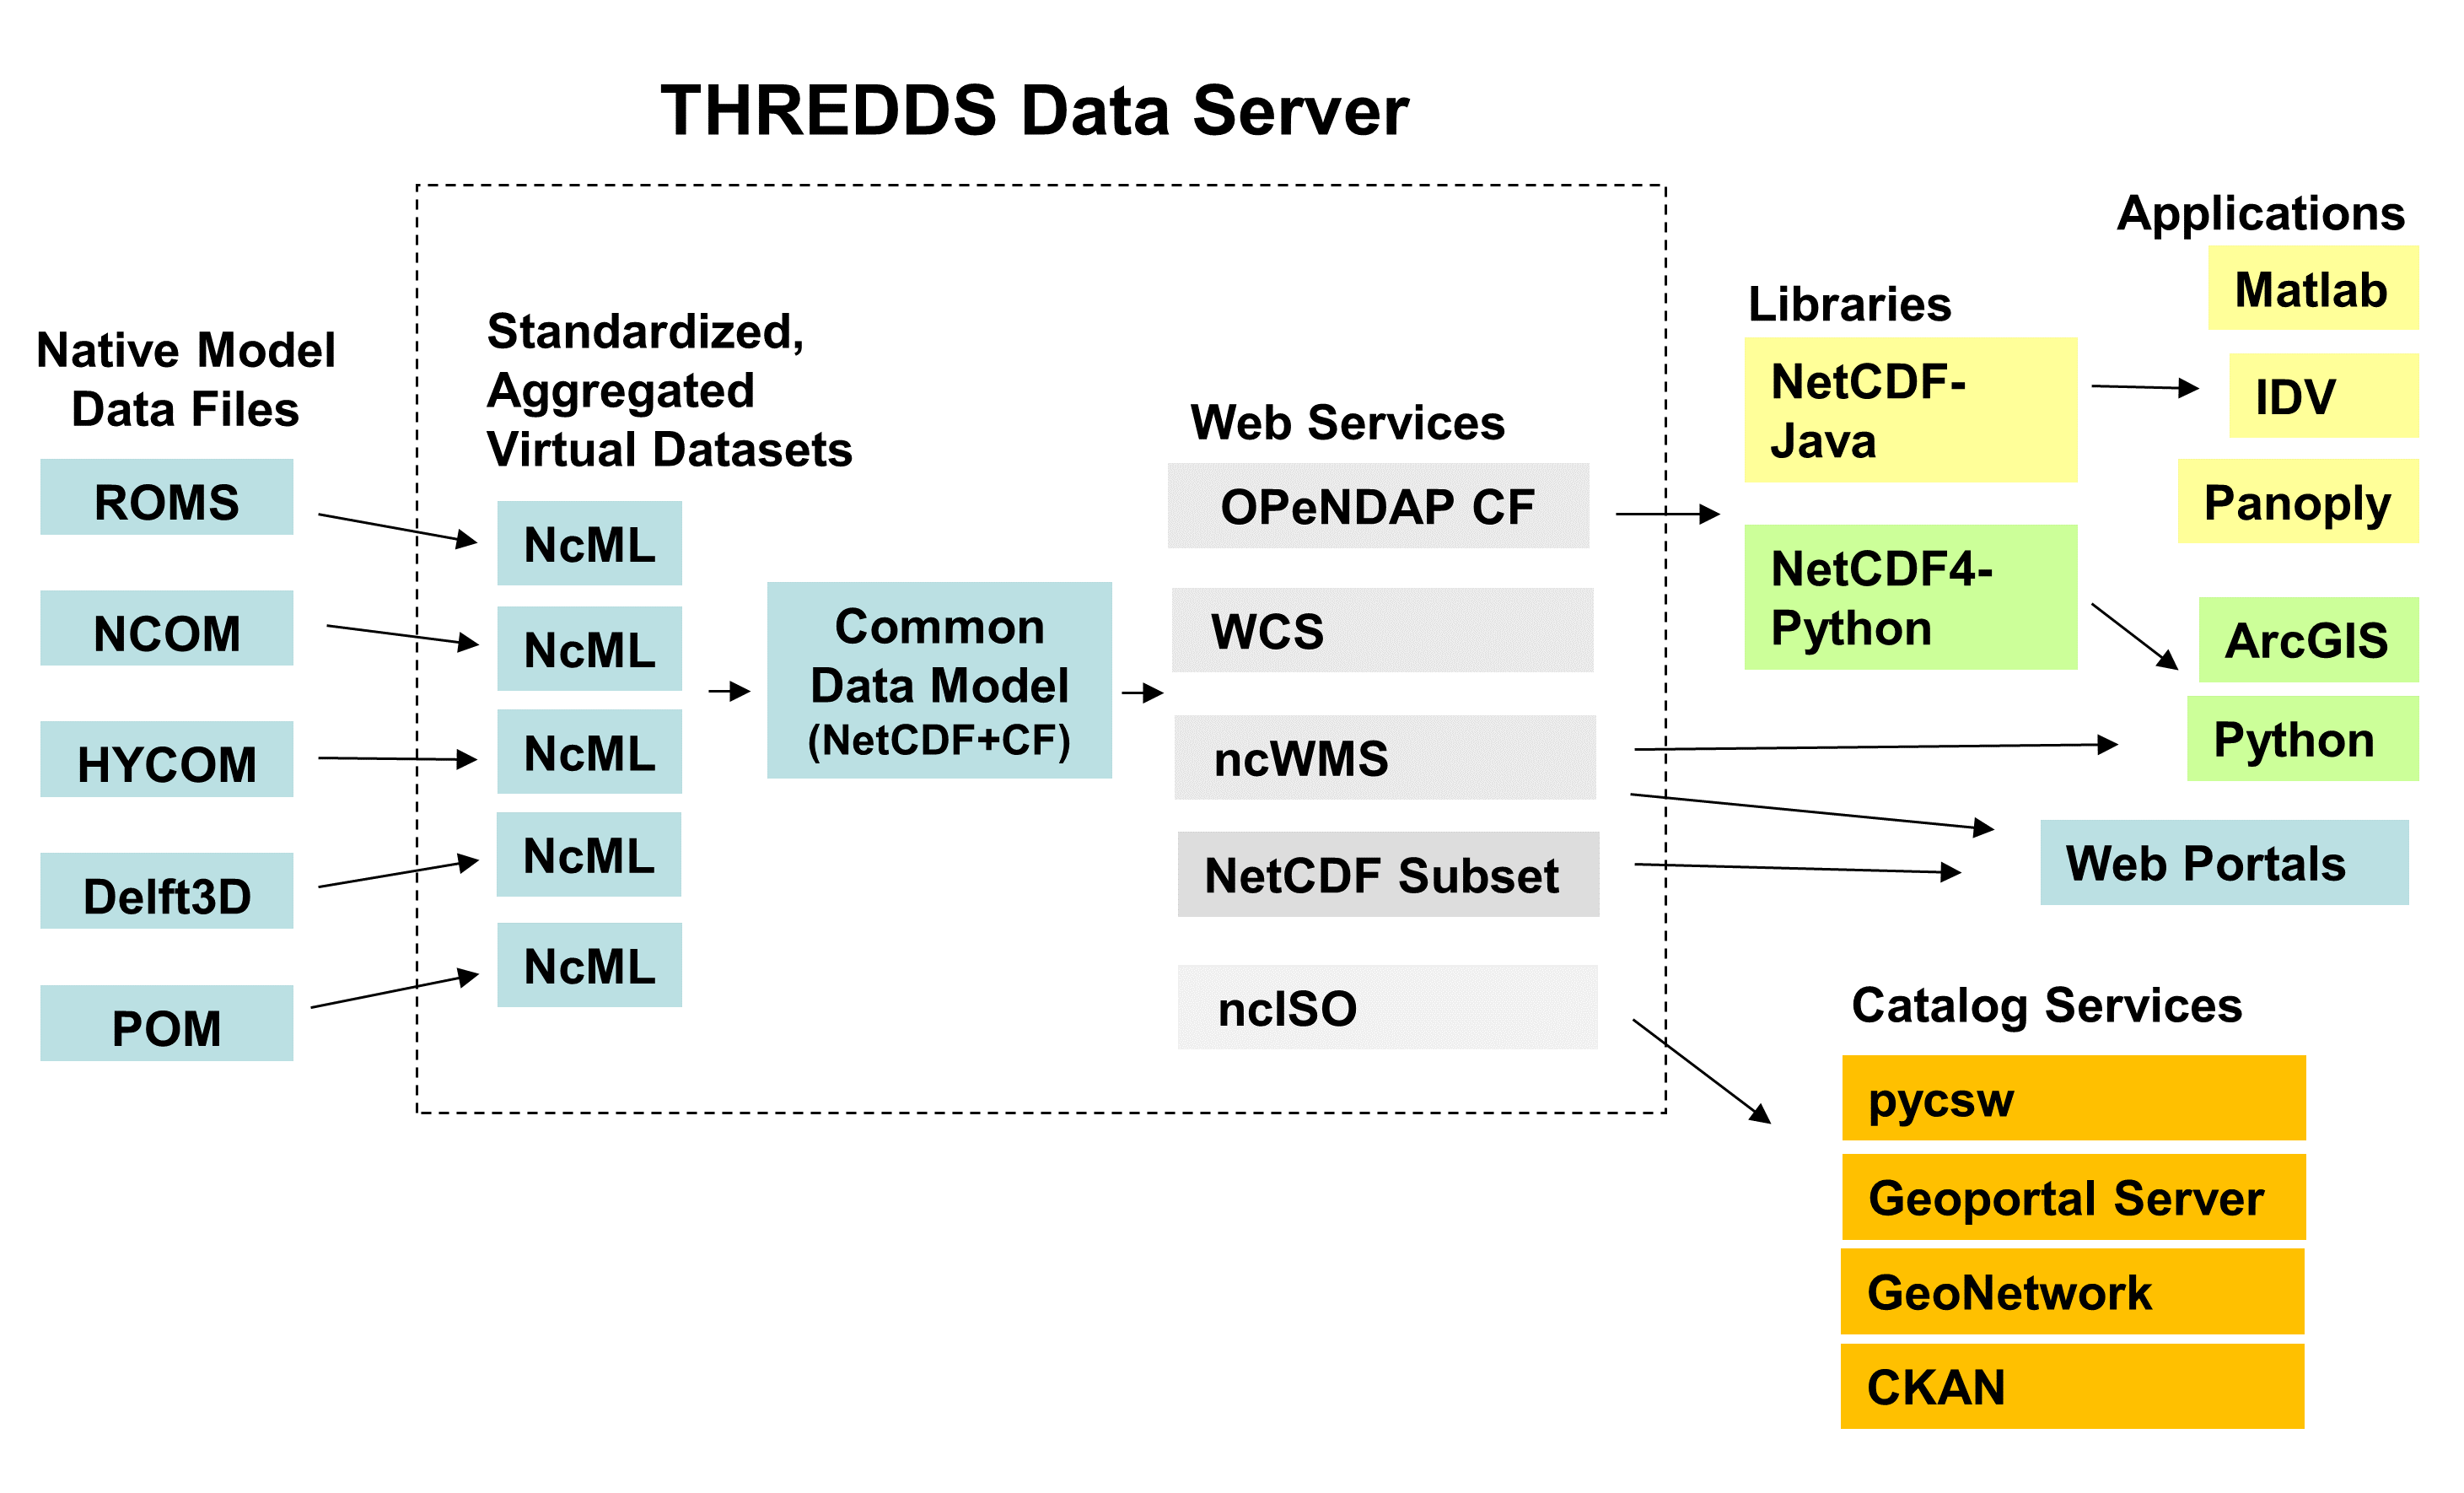
\includegraphics[width=130mm]{framework_slide.png}
\caption{The IOOS Model Data Framework.  Collections of non-standard NetCDF (or GRIB) files are transformed via NetCDF Markup Language (NcML) into aggregated, standardized datasets that can be represented internally in the THREDDS Data Server in a common data model.  This data in common form can then be delivered via a number of standard services, including map services (WMS), data services (OPeNDAP, WCS and NetCDF Subset Service), and metadata services (ncISO).  This services in turn feed web portals, scientific analysis workflows in Python or Matlab,  and catalog services. }
\label{osd-2015-0064-f00.pdf}
\end{figure}


\begin{figure}
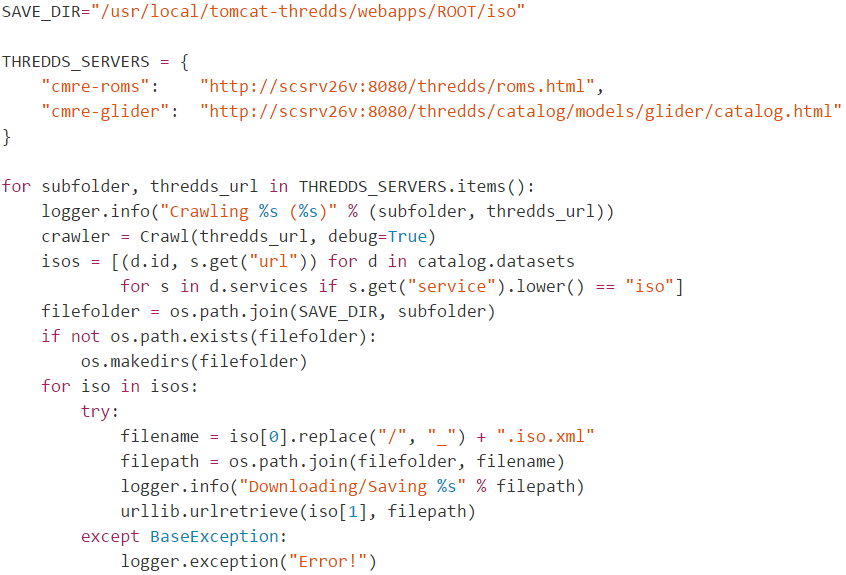
\includegraphics[width=130mm]{os-2015-64-discussions-f01.png}
\caption{Snippet of Python code to crawl THREDDS catalogs. This code
  crawls two catalogs that contain forecast model runs and glider
  data. \copyright~North Atlantic Threaty Organization, all rights reserved. Provided by STO-CMRE (\url{www.cmre.nato.int}).}
\label{osd-2015-0064-f01.pdf}
\end{figure}


\begin{figure}
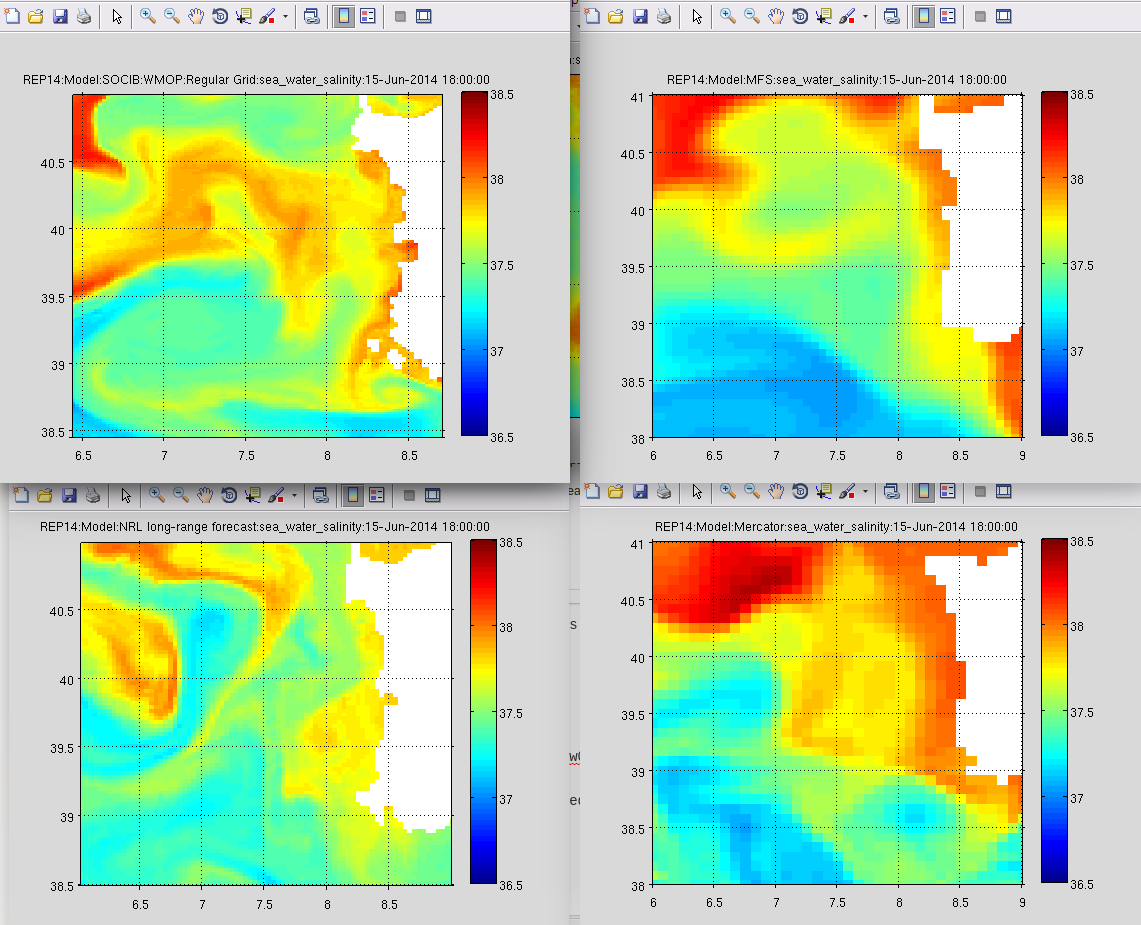
\includegraphics[width=120mm]{os-2015-64-discussions-f03.png}
\caption{Comparison of surface salinity snapshots from four different
  models during REP14-MED Field Trial. By delivering data via web
  services with CF conventions, and using NCTOOLBOX which understands
  CF conventions, these figures were able to be made without any
  model-specific code.  \copyright~North Atlantic Threaty
  Organization, all rights reserved. Provided by STO-CMRE.}
\label{osd-2015-0064-f03.pdf}
\end{figure}

\begin{figure}
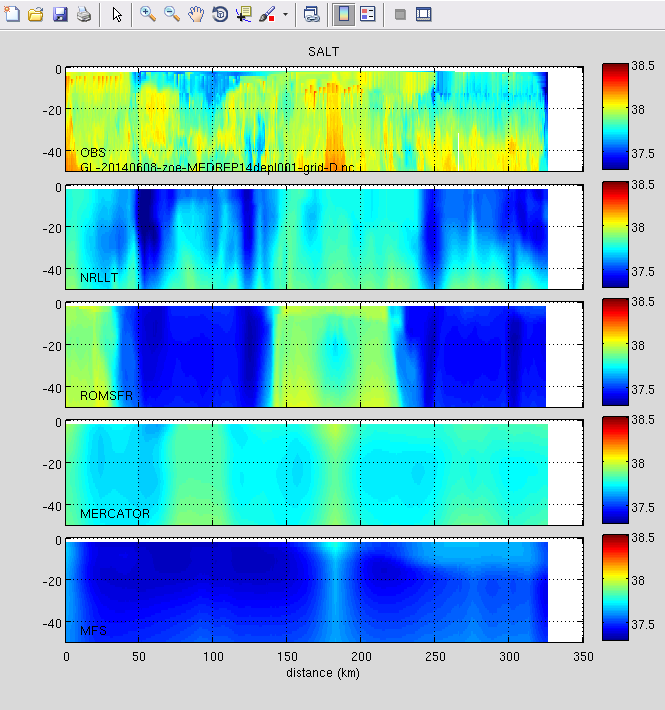
\includegraphics[height=110mm]{os-2015-64-discussions-f04.png}
\caption{Vertical sections of salinity data from an ocean glider
  compared with virtual glider paths through four numerical
  models. Use of CF Conventions and NCTOOLBOX allowed the vertical
  coordinates from these four different models to be computed without
  any model-specific code.  \copyright~North Atlantic Threaty
  Organization, all rights reserved. Provided by STO-CMRE.}
\label{osd-2015-0064-f04.pdf}
\end{figure}

\begin{figure}
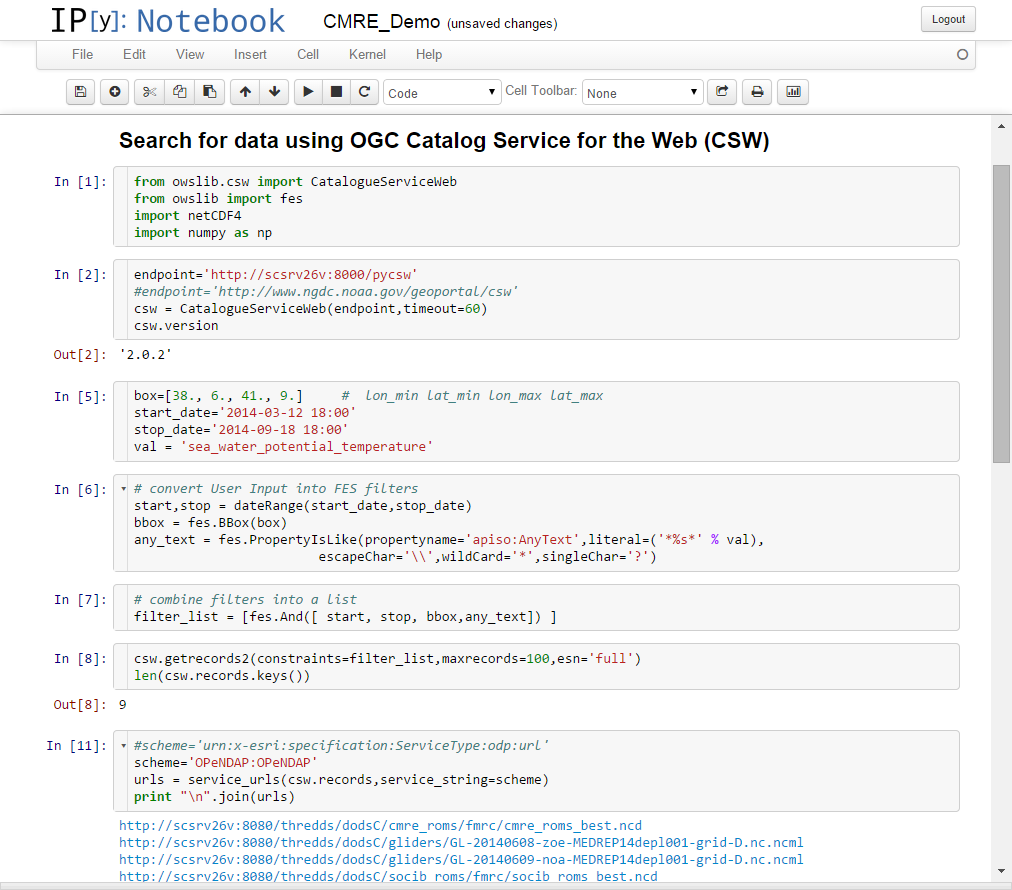
\includegraphics[width=125mm]{os-2015-64-discussions-f05.png}
\caption{A~snippet from an IPython Notebook demo, demonstrating
  a~geospatial, temporal and free-text search for data using the
  owslib package to construct CSW queries and parse the results. Nine
  records are found, and the OPeNDAP data endpoints are then selected,
  from which data can be extracted in a~common way, since CF
  Conventions are used. \copyright~North Atlantic Threaty
  Organization, all rights reserved. Provided by STO-CMRE.}
\label{osd-2015-0064-f05.pdf}
\end{figure}

\begin{figure}
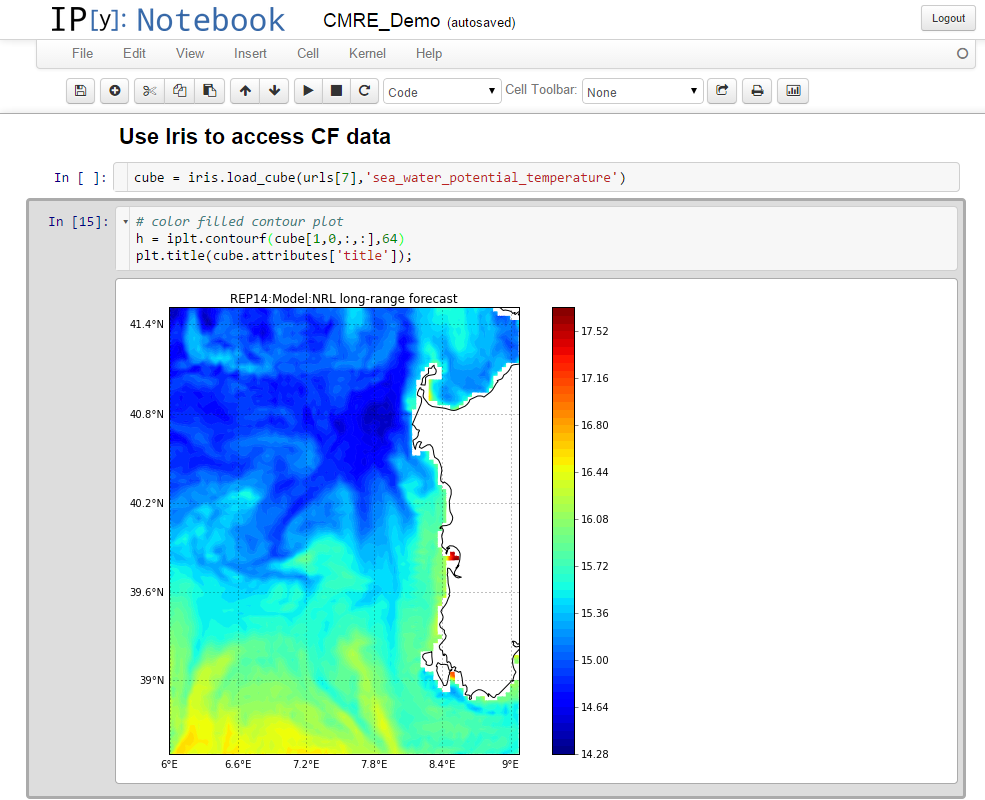
\includegraphics[width=130mm]{os-2015-64-discussions-f06.png}
\caption{Another snippet from the Ipython Notebook demo, extracting
  data from one of the discovered OPeNDAP URLs using the Iris
  package. \copyright~North Atlantic Threaty Organization, all rights reserved. Provided by STO-CMRE.}
\label{osd-2015-0064-f06.pdf}
\end{figure}

\begin{figure}
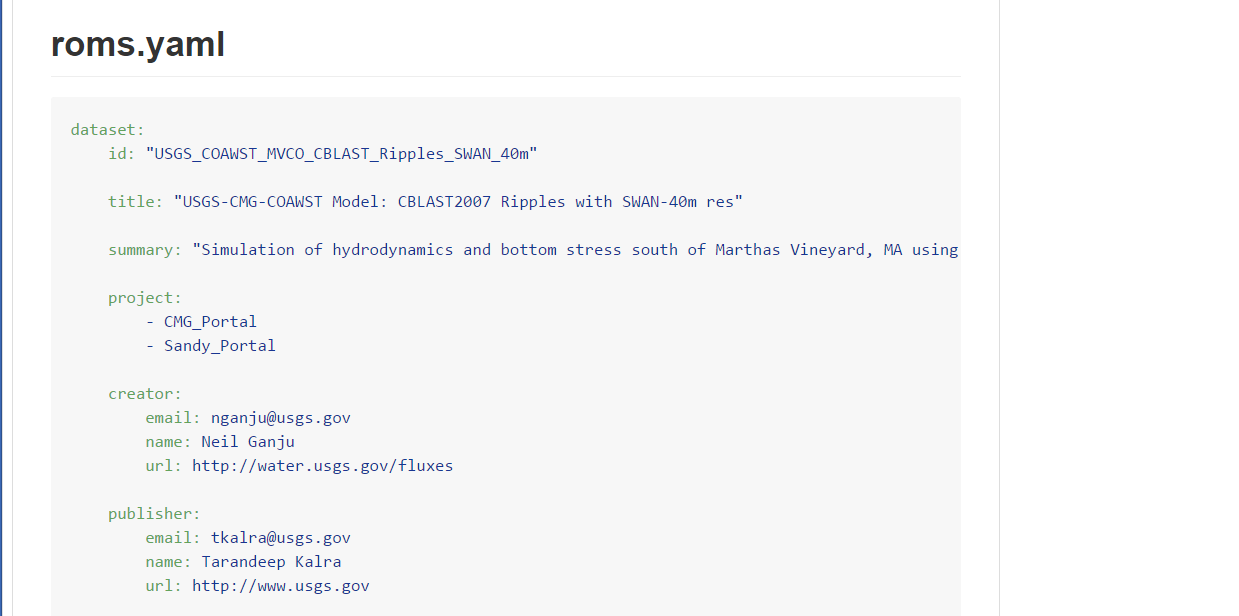
\includegraphics[width=140mm]{os-2015-64-discussions-f07.png}
\caption{Example of a~YAML file, created by the modeller, and used to
  specify simulation specific parameters. This YAML file is converted
  into NcML using the yaml2roms python script. By specifying
  ``CMG\_Portal'' in the Project section, the modeller is indicating
  that this dataset should be included in the USGS CMG\_Portal web
  application.}
\label{osd-2015-0064-f07.pdf}
\end{figure}

\begin{figure}
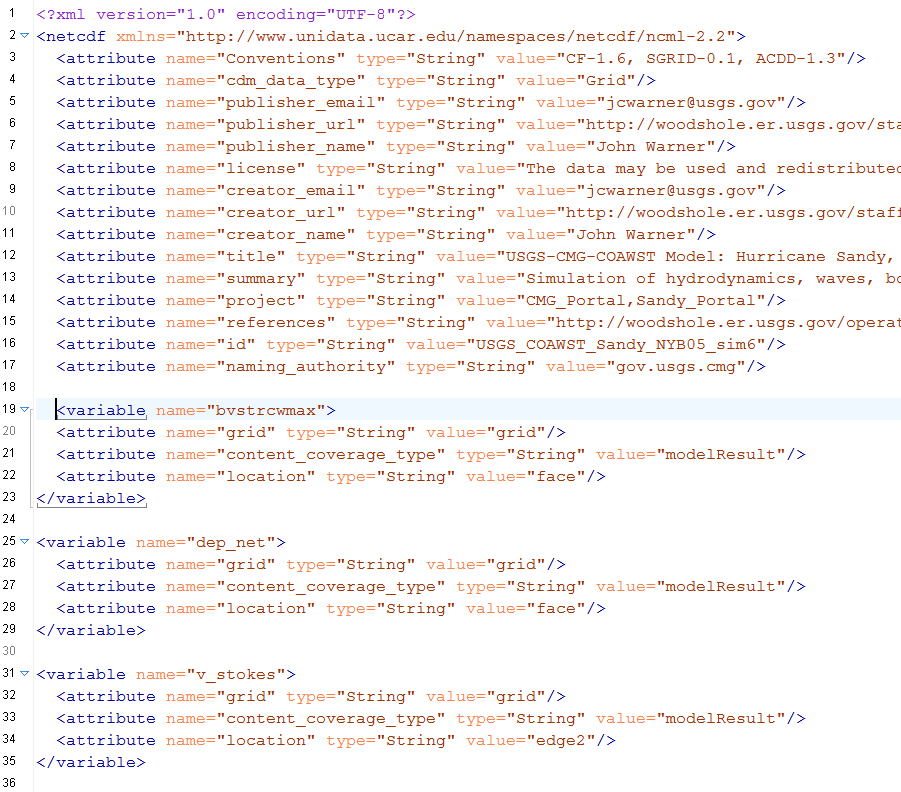
\includegraphics[width=130mm]{os-2015-64-discussions-f08.png}
\caption{A~sample NcML file produced by the yaml2ncml.py python
  script.  Although these files can be created by hand using a~text
  editor, getting validated NcML has proven difficult for modeller,
  and the yaml2ncml pathway has been found to be less
  error-prone. This NcML file not only specifies attributes, but also
  contains a~regular expression that specifies which NetCDF files
  should be part of this aggregated dataset (not shown).}
\label{osd-2015-0064-f08.pdf}
\end{figure}

\begin{figure}
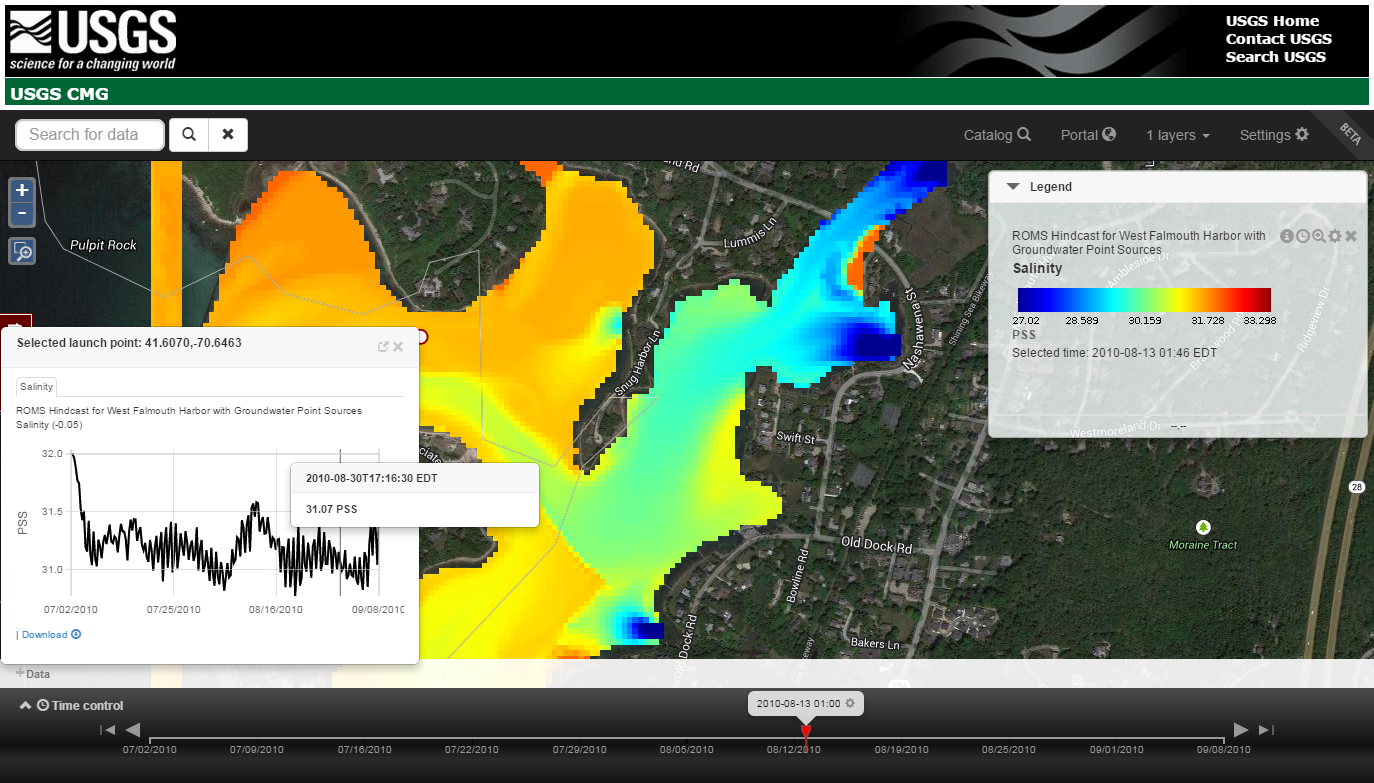
\includegraphics[width=145mm]{os-2015-64-discussions-f09.png}
\caption{Viewing a~USGS CMG dataset in the CMG\_Portal web
  application. The map is made by a~dynamic request to the WMS service
  provided by the THREDDS Data Server. The user has clicked a~location
  on the map, which extracts a~time series at that location using the
  WMS \textit{getFeatureInfo} response. }
\label{osd-2015-0064-f09.pdf}
\end{figure}

\begin{figure}
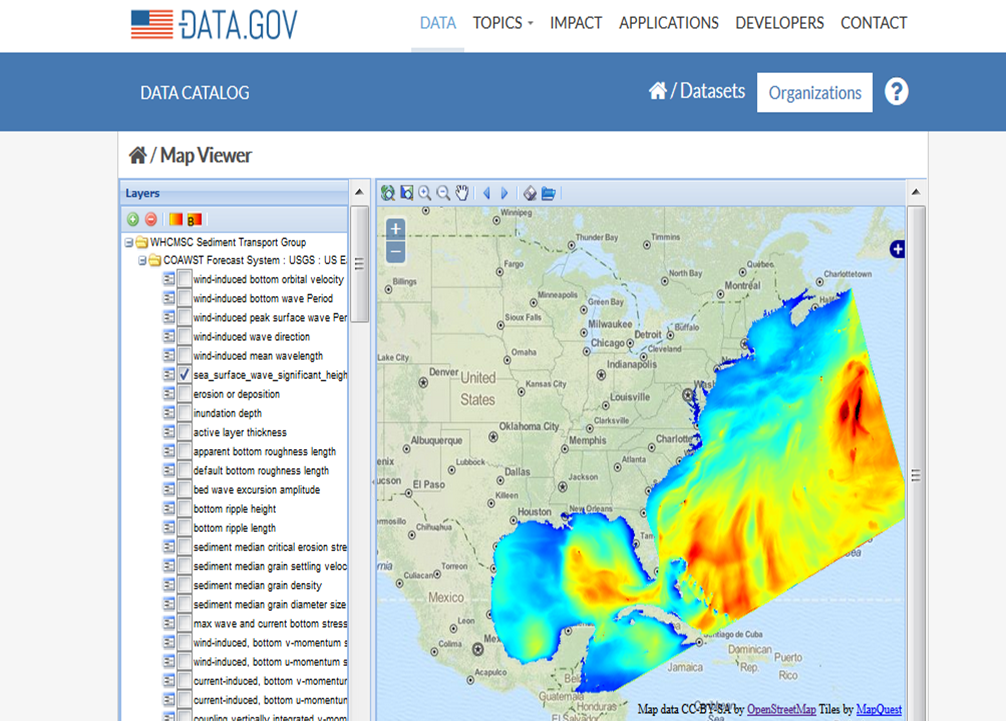
\includegraphics[width=140mm]{os-2015-64-discussions-f10.png}
\caption{Viewing a~discovered USGS CMG dataset in the Data.gov
  built-in Map Viewer application. The Map Viewer is requesting this
  image from the WMS service built into the THREDDS Data Server. }
\label{osd-2015-0064-f10.pdf}
\end{figure}

\begin{figure}
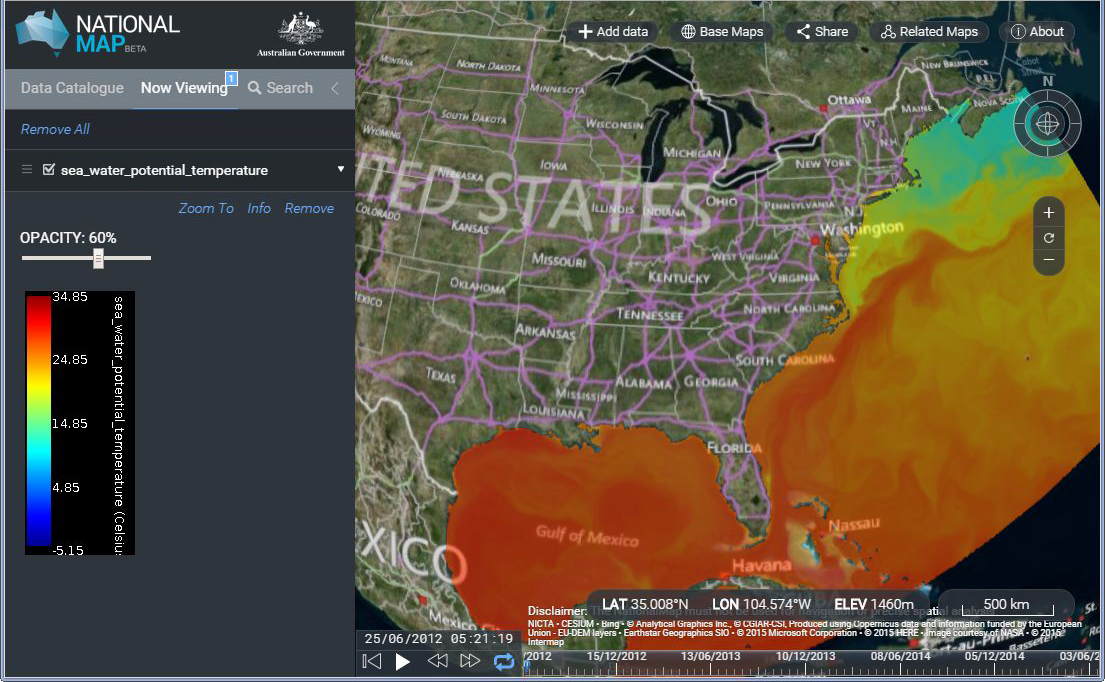
\includegraphics[width=145mm]{os-2015-64-discussions-f11.jpg}
\caption{USGS CMG dataset displayed on the Australian National Map
  application. This map application is also requesting the image from
  the WMS service provided by the THREDDS Data Server.}
\label{osd-2015-0064-f11.pdf}
\end{figure}

\end{document}

\endinput
